\section{Introduction}

Small UAS carrying LiDAR, RGBD cameras, or monocular cameras using Structure from Motion (SfM) can generate 3D point clouds of nearby landing sites. Polylidar3D can transform these dense point clouds to polygonal representations of flat-surfaces in real-time while accounting for obstacles. Chapter \ref{ch:landingsim} presented simulation results using Polylidar3D for real-time touchdown point selection for rooftops using on-board LiDAR and cameras. This chapters extends this simulation work to real-world experiments carried out at the University of Michigan Flight Lab. This work demonstrates integrating multiple LiDAR scans into a larger cohesive mesh in which noise is reduced. The final mesh is then sent to Polylidar3D for polygon extraction and touchdown point selection.

We assembled a sensor-package that holds an Intel RealSense L515 LiDAR, RealSense T265 Tracking Camera, and an Odyseey x86 \acf{SBC}. Together they provide color/depth images, 6DOF tracking, and the computation power needed to implement our landing zone selection methods presented in Chapter \ref{ch:landingsim}. Safe touchdown points are found in an obstacle cluttered indoor environment. Two separate experiments are performed: one with the sensor package hand carried and the other with the package mounted underneath a flying quadrotor.  Results indicate that our presented methods are able to identity safe touchdown points accurately and efficiently.

\section{Touchdown Point Selection}\label{sec:ch7_volume_integration}

Chapter \ref{ch:landingsim} proposed our method of selecting a touchdown point from a single scan of a rotating LiDAR sensor mounted underneath a drone. The single range image is quickly transformed into a mesh of the environment.  This chapter proposes to alternatively integrate multiple scans together to create a unified mesh of the environment. This integration process requires the drone to have precise localization capabilities. This capability is provided by the Intel RealSense T265 tracking sensor and mounted on-board the drone. 

The L515 LiDAR is able to produce an \ac{RGBD} image by aligning both the depth and color data streams. Multiple \ac{RGBD} frames are integrated into a cohesive map using methods from Zhou et al.~\cite{zhou_dense_2013} and implemented in Open3D~\cite{zhou_open3d_2018}. The technique works by creating a truncated signed distance field within a voxel volume.  The volume is updated by deprojecting points from an RGBD image into the volume which requires both the intrinsics and extrinsic of the camera. The signed distance field is then extracted as a triangular mesh using the marching cubes algorithm \cite{10.1145/37401.37422}.  In this work we use a voxel size of 5cm which provides more than enough resolution for landing site decisions. At 3m of distance the range noise of the L515 LiDAR is less than 1cm \cite{nxp:tja1043} and is nearly removed after integrating multiple frames.

After the mesh is extracted, Polylidar3D is used to extract all the flat surfaces as polygons. Any obstacles embedded on the surface are captured as interior holes. The largest inscribed circle of the largest polygon is used to select a landing zone.  A circle must meet the minimum radial footprint of 0.75 meters, determined by quadrotor size, or no touchdown point is selected. We develop an open-source hardware and software platform that implements all of these functionalities and validate it experimentally.

% and validated by a motion capture system

\section{Experimental Setup}

\subsection{Sensor Package Construction}

The sensor package is shown in Figure \ref{fig:ch7_sensor_package_pic}. The package is composed of a (1) RealSense L515 LiDAR/Color Sensor, (2) RealSense T265 Tracking Camera, (3) Odyseey x86 \ac{SBC}, and a (4) 12V Li-ion battery pack. The package is held together with 3D printed plates and standoffs with a total weight of 720 grams. The dimensions of the package are $120 \times 110 \times 50 mm$. The L515 device is mounted directly underneath the sensor package pointing down, while the T265 is mounted in the front. The Odyseey \ac{SBC} and battery back are placed between the printed plates.

\begin{figure}[!htb]
  \centering
  \begin{subfigure}[t]{.40\linewidth}
    \centering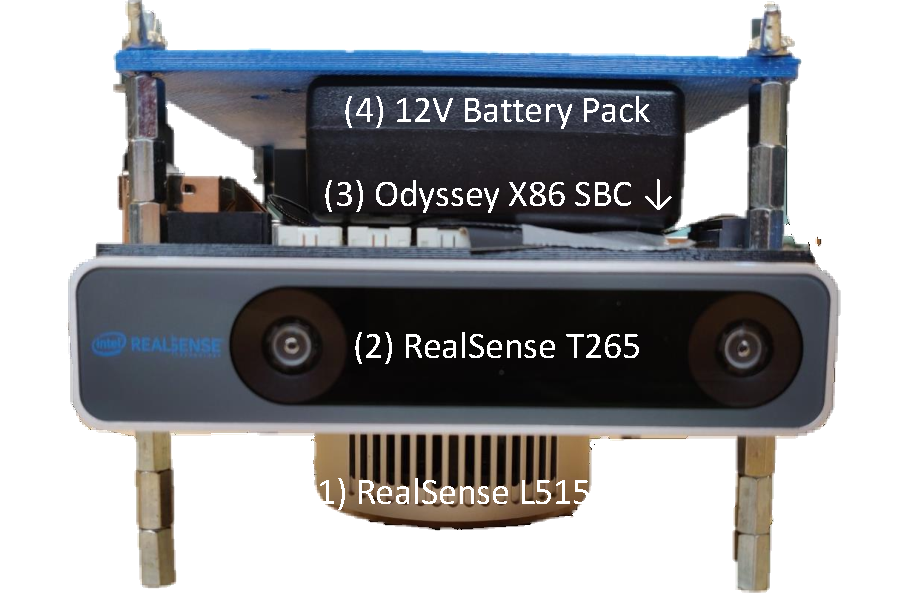
\includegraphics[page=1,clip,trim=0cm 0cm 0cm 0cm,width=.99\linewidth]{chapter_7_experiments/imgs/sensor_package.pdf}
    \caption{\label{fig:ch7_sensor_package_a}Front View}
  \end{subfigure}
  \begin{subfigure}[t]{.40\linewidth}
    \centering\includegraphics[page=3,clip,trim=0cm 0cm 0cm 0cm,width=.99\linewidth]{chapter_7_experiments/imgs/sensor_package.pdf}
    \caption{\label{fig:ch7_sensor_package_b}Underside View}
  \end{subfigure}
  \caption[Sensor package components]{Sensor Package Components}\label{fig:ch7_sensor_package_pic}
\end{figure}

\subsection{Sensor Coordinate Frames}

The coordinate frames of the L515 LiDAR and T265 tracking sensors are shown in Figure \ref{fig:ch7_sensor_frames} and denoted as \{L\} and \{T\}, respectively. The L515 follows nominal camera axes conventions (z-axis forward, x-axis right) while the tracking sensor follows \acf{VR} conventions (z-axis backwards, x-axis right). The T265 outputs a 6DOF pose (position and orientation) with respect to a world frame origin denoted \{WT\} that is set during initialization. As a result \{WT\} follows \ac{VR} axes conventions which is non-standard in aerospace applications. Another world frame \{WNED\} is created to be coincident to \{WT\} but rotated such that it follows NED conventions (z-axis down, x-axis forward). The reference frame of data will be indicated by a superscript, e.g., $\mathcal{P}^{L}$ denotes a point cloud in the LiDAR frame. An homogeneous transformation between frame A to frame B is denoted $\mathbf{H}^A_B$.

\begin{figure}[!htb]
  \centering
  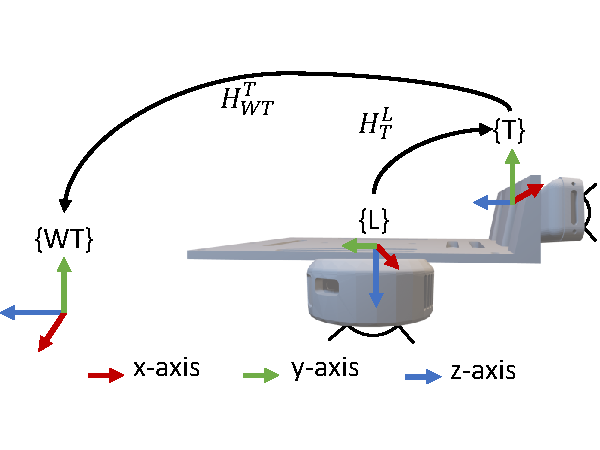
\includegraphics[page=1,clip,trim=0cm 1cm 0cm 1cm,width=.45\linewidth]{chapter_7_experiments/imgs/sensor_frames.pdf}
  \caption[Sensor package coordinate frames]{Sensor Package Coordinate Frames}\label{fig:ch7_sensor_frames}
\end{figure}
Volume integration as described in Section \ref{sec:ch7_volume_integration} requires the LiDAR camera intrinsics and extrinsics. The intrinsics of the L515 are factory calibrated and provided by the RealSense SDK \cite{noauthor_github_2020-4}. The T265 pose provides the extrinsics $\mathbf{H}^{T}_{WT}$  of the T265 sensor with respect to \{WT\}. This pose must be appropriately transformed to create the extrinsics of the L515 camera in the world NED frame:
\begin{align*}
   \mathbf{H}^{L}_{WNED}  =  \mathbf{R}^{WT}_{WNED} \cdot \mathbf{H}^{T}_{WT} \cdot \mathbf{H}^{L}_{T}
\end{align*}
where $\mathbf{R}^{WT}_{WNED}$ denotes the rotation between \{WT\} to \{WNED\}. The matrix $\mathbf{H}^{L}_{WNED}$ may then transform points in \{L\} to \{WNED\} to create a mesh in this reference frame.

\subsection{Drone Frame and Sensor Package Integration}

We utilize the M330 quadrotor designed at UMICH A2SYS Lab for all flight experiments \cite{romano_experimental_2019}. The frame measures 33cm diagonally between each pair of motors and is powered by a 4S 3000mAh LiPo battery. Markers are placed on the drone frame and tracked by a \ac{MCS}. The \ac{MCS} sends pose estimates of the drone to the flight controller using a wireless serial radio. The drone is controlled by a custom autopilot running on a BeagleBone Blue that uses these ground truth pose estimates for position and yaw control. The sensor package is mounted directly underneath the drone as shown in Figure \ref{fig:ch7_drone_frame}. The total weight of the drone and sensor package is 1720 grams.

\begin{figure}[!htb]
  \centering
  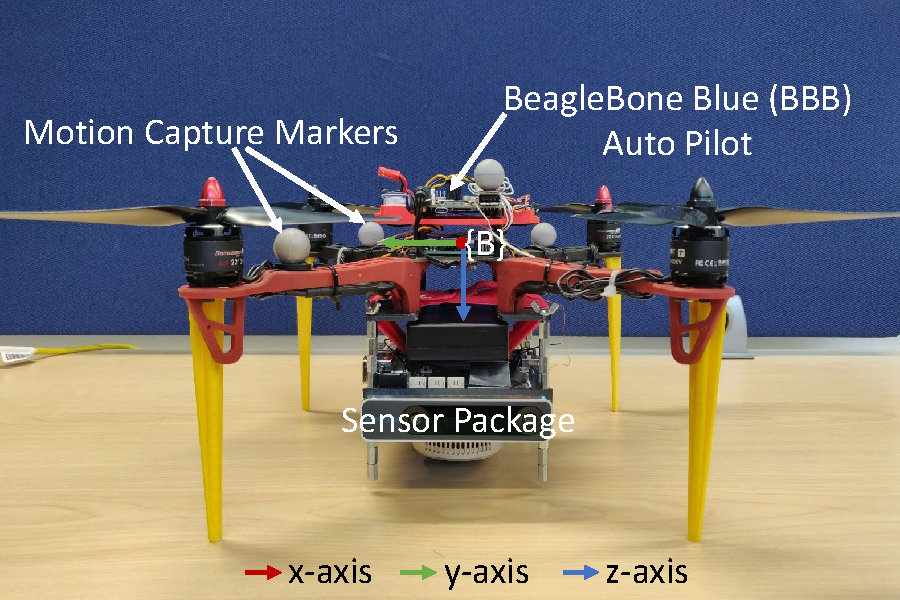
\includegraphics[page=1,clip,trim=0cm 0cm 0cm 0cm,width=.50\linewidth]{chapter_7_experiments/imgs/drone_with_sensor_package.pdf}
  \caption[Sensor package mounted underneath drone]{The sensor package is mounted directly underneath the drone. The beagle bone blue autopilot, motion capture markers, and drone body frame \{B\} are indicated.}\label{fig:ch7_drone_frame}
\end{figure}

We continue to use the \ac{MCS} for drone position control because the T265 sensors accuracy, precision, and reliability have note been fully tested for flight experiments. The T265 is only used to generate a mesh of the environment to give a final touchdown point command to the drone. Note that the T265 sensor initializes the \{WNED\} frame during startup. Therefore the drone is positioned such that the \ac{MCS} coordinate frame is aligned with \{WNED\} before every flight. However, there will be a marginal height offset ($<$ 10cm) between these frames because the T265 is mounted higher than the ground plane. All commanded touchdown points will be given in the \{WNED\} frame.

\subsection{Environment}

All experiments were performed inside the University of Michigan's Ford Robotics Building Flight Lab. Four obstacles were placed on the floor including three boxes and one small ladder. The environment, obstacle labelling, and origin frame are shown in Figure \ref{fig:ch7_workspace_a}. Each obstacle dimensions were measured using a ruler and placed at known positions within the environment to create a ground truth overlay shown in Figure \ref{fig:ch7_workspace_b}. The workspace was limited to a $4m\times3.5m$ box centered at the \ac{MCS} origin and represents the safely navigable region for the drone. Together the workspace and obstacles form a ground truth polygon to assess the accuracy of any proposed landing area created by Polylidar3D.

\begin{figure}[!htb]
  \centering
  \begin{subfigure}[t]{.50\linewidth}
    \centering  \includegraphics[page=2,clip,trim=0cm 1cm 0cm 0cm,width=.99\linewidth]{chapter_7_experiments/imgs/ExperimentSetup.pdf}
    \caption{\label{fig:ch7_workspace_a}}
  \end{subfigure}
  \begin{subfigure}[t]{.35\linewidth}
    \centering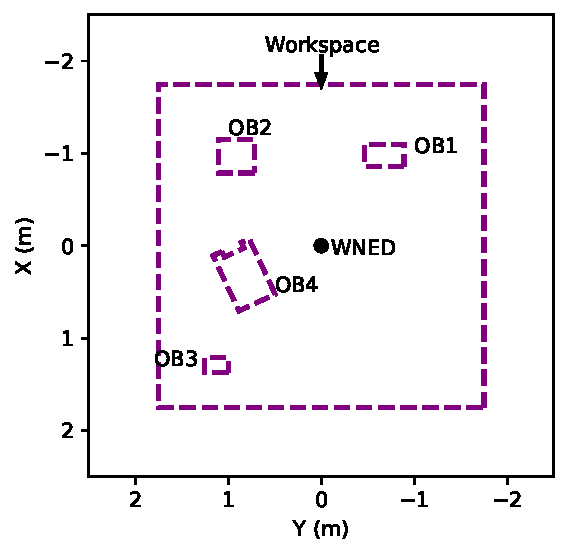
\includegraphics[page=1,clip,trim=0cm 0cm 0cm 0cm,width=.99\linewidth]{chapter_7_experiments/imgs/workspace_plot.pdf}
    \caption{\label{fig:ch7_workspace_b}}
  \end{subfigure}

  \caption[Photo of flight lab and obstacle placement]{(\subref{fig:ch7_workspace_a}) Photo of flight lab and obstacle placement. (\subref{fig:ch7_workspace_b}) Ground truth measurement of environment}\label{fig:ch7_workspace}
\end{figure}

\subsection{Hardware and Software Integration}\label{sec:ch7_software}

The data streams and frequencies for each sensor are shown in Table \ref{table:ch7_datastreams}. Because of the real-time computational demand of integrating RGBD frames into a volume the frequency of the L515 was reduced to 6Hz. However, the authors noticed no degradation in mesh quality in comparison to running at full speed (30Hz) on a desktop computer. The resolution of the depth stream and RGB stream were set at the recommended levels from Intel to further reduce computational demand. 


\begin{table}[ht]
\centering
\caption[Sensor Package]{Sensor Package Details}
\label{table:ch7_datastreams}
\begin{tabular}{@{}llll@{}}
\hline\noalign{\smallskip}
Sensor                                       & Stream & Frequency  & Description                             \\ 
\noalign{\smallskip}\hline\noalign{\smallskip}
\multirow{2}{*}{L515 LiDAR Camera}           & Depth    & 6 Hz & 640X480, Depth Stream      \\
                                             & Color    & 6 Hz    & 1280X720, RGB Stream                      \\
\multirow{1}{*}{T265 Tracking Camera}         & 6DOF    & 100 Hz & Position and Orientation                         \\
\noalign{\smallskip}\hline\noalign{\smallskip}
\end{tabular}
\end{table}


Figure \ref{fig:ch7_software} shows a diagram of the devices and software used in the experiments. The top left of the diagram displays the hardware interfaces, the top right is a legend, and the bottom is the software architecture. The Odyssey \ac{SBC} communicates to the drone flight controller (BBB) through a serial connection. The communication is one-way and allows the emergency landing software to command a landing position. Currently the command is issued only once, cannot be cancelled, and the drone will immediately fly a constant altitude path to the position and then land. 

The software is composed of four main programs: \texttt{RS-Pub}, \texttt{RS-Integrate}, \texttt{Landing Sever}, and \texttt{Record}. Programs communicate with each other with messages using \ac{ECAL}, a fast publish-subscribe middleware that manages inter-process communication \cite{Continental_Github_ecal}. The program \texttt{RS-Pub} is responsible for configuring and gathering data from the RealSense devices and publishes shared memory messages containing \ac{RGBD} frames with pose information. The program \texttt{RS-Integrate} subscribes to these messages and will integrate them into a cohesive voxel volume using Open3D \cite{zhou_open3d_2018}. It also runs a TCP/IP server that upon request will extract a mesh from the volume. The program \texttt{Landing-Sever} contains all the algorithms and software previously presented in Chapter \ref{ch:landingsim} for real-time touchdown point selection. This contains our own algorithms and software such as mesh smoothing, polygon extraction, polygon filtering, and touchdown point selection. This program also runs an interactive terminal user interface, shown in Figure \ref{fig:ch7_tui}, which allows a user to activate the emergency landing protocols. Finally, the program \texttt{Record} efficiently records all messages with synchronized timestamps. All code for this work is open-source and freely available \cite{Castagno_Github_realsensepackage}.

\begin{figure}[!tb]
    \centering  
    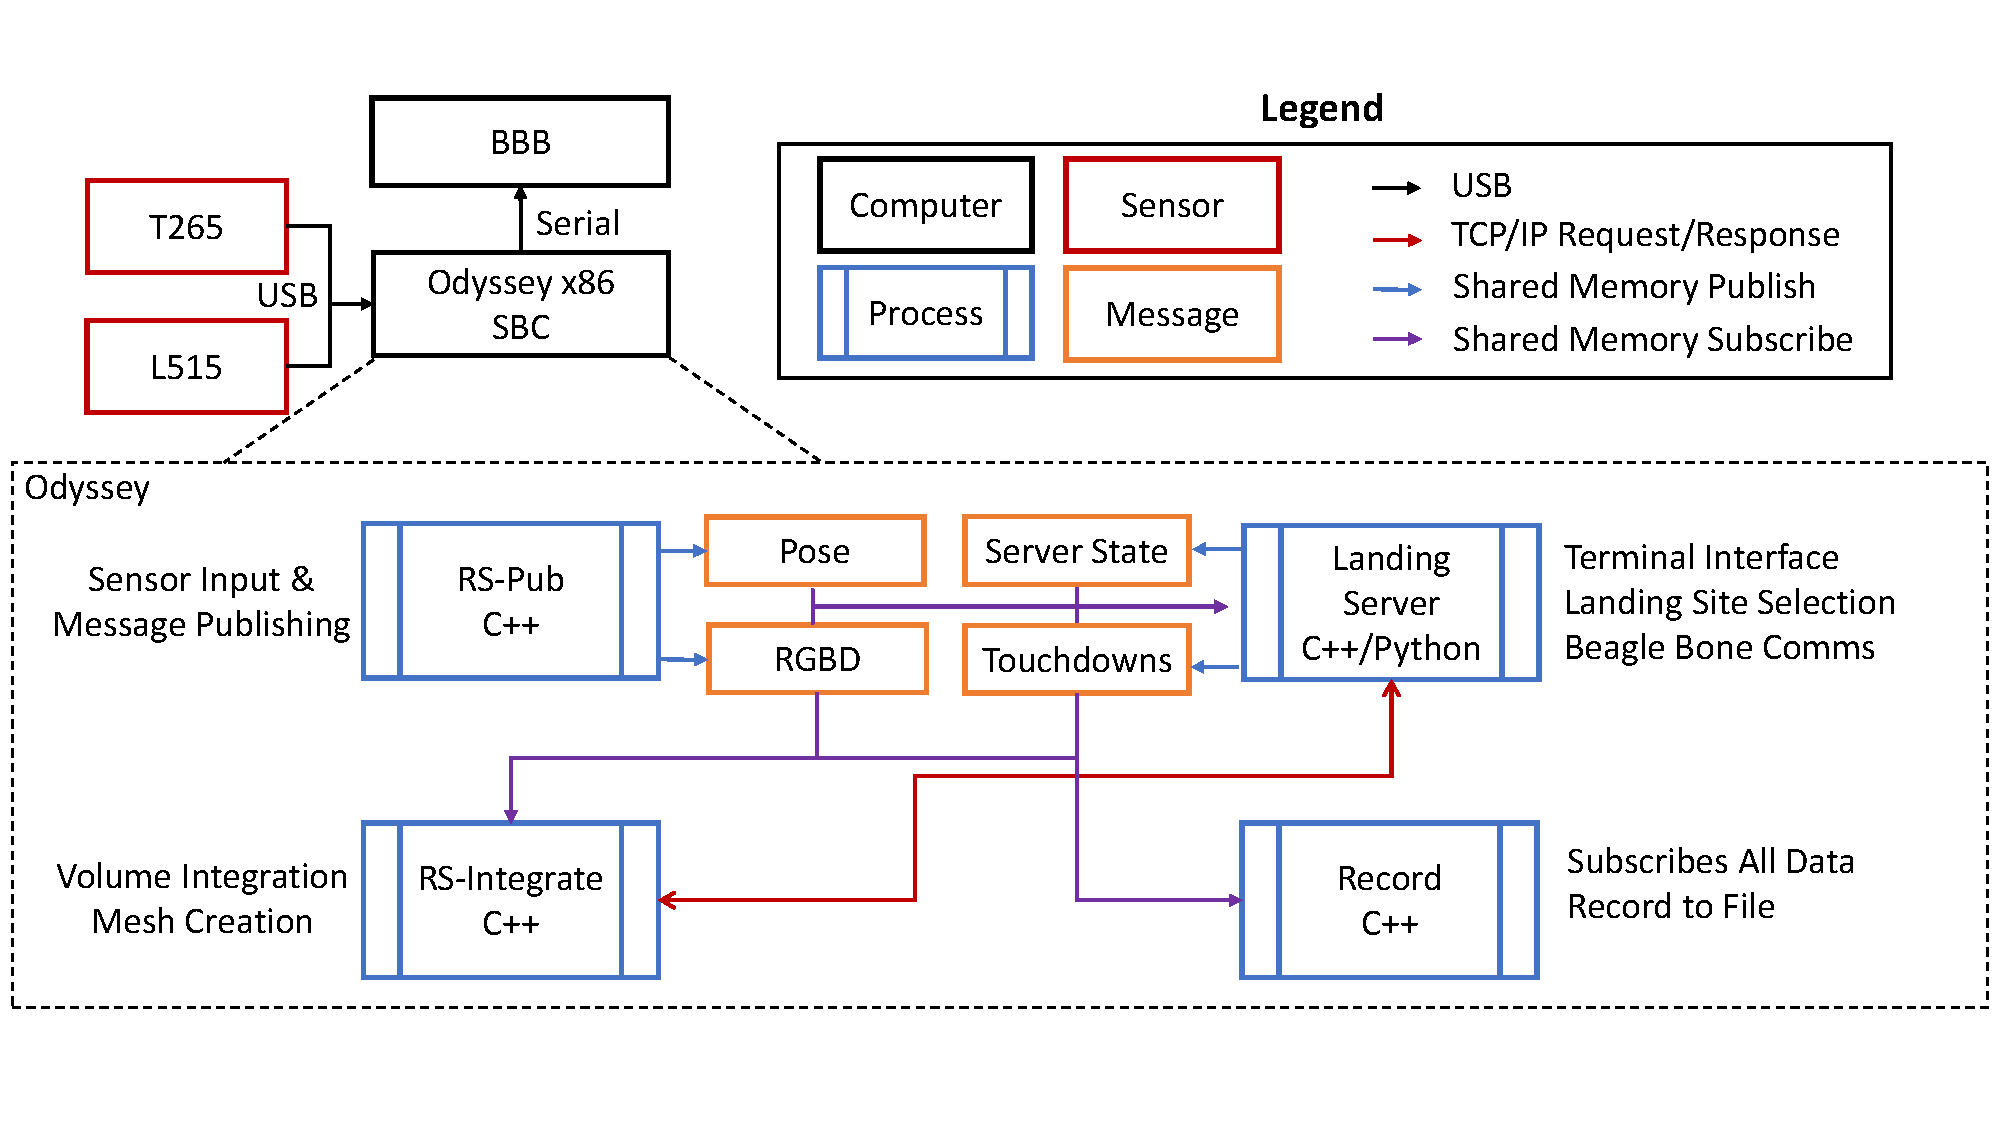
\includegraphics[page=1,clip,trim=0cm 0cm 0cm 0cm,width=.95\linewidth]{chapter_7_experiments/imgs/SoftwareOverview.pdf}
    \caption[Overview of hardware interfaces and software architecture]{Overview of Software Architecture}\label{fig:ch7_software}
\end{figure}

\begin{figure}[!tb]
    \centering  
    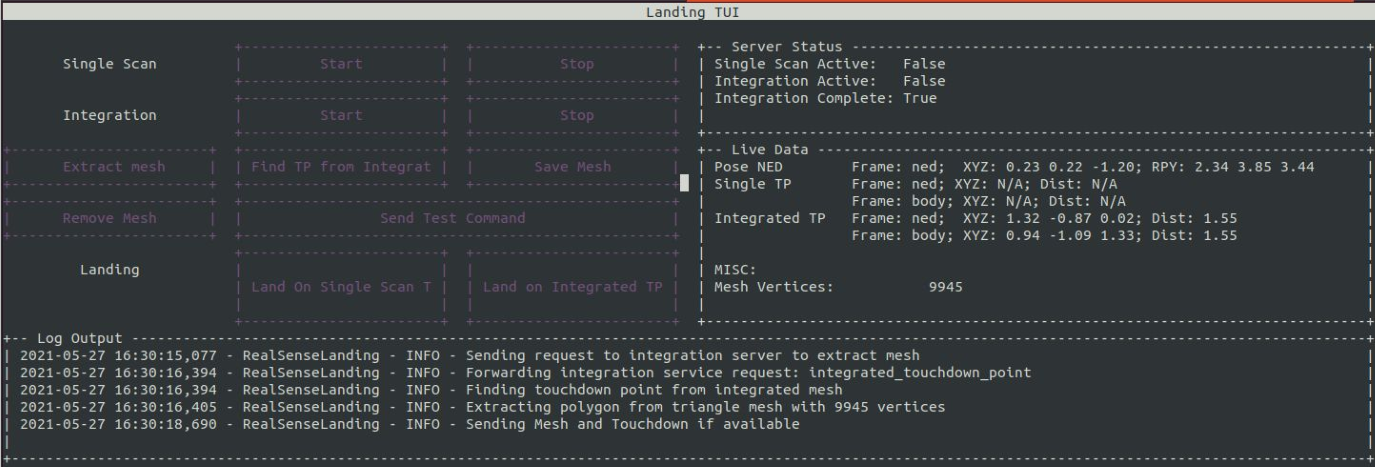
\includegraphics[page=1,clip,trim=0cm 0cm 0cm 0cm,width=.95\linewidth]{chapter_7_experiments/imgs/SensorPackage_TUI.pdf}
    \caption[Picture of terminal user interface for emergency landing]{Picture of terminal user interface for emergency landing}\label{fig:ch7_tui}
\end{figure}

\section{Results}

Section \ref{sec:ch7_results_handcarry} and \ref{sec:ch7_results_flight} presents results for hand-carry and flight tests, respectively. Section \ref{sec:ch7_results_execution_time} provides execution timing results while Section \ref{sec:ch7_results_t265_accuracy} presents accuracy results of the T265.

\subsection{Hand Carry Test} \label{sec:ch7_results_handcarry}

Five hand-carry tests were performed in the Flight Lab. An identical software suite as presented in Section \ref{sec:ch7_software} was running except serial landing commands to the drone were disabled. To simulate flight, we attached an extendable pole to the sensor package.  The package was then picked up and moved around in a box pattern within the environment. The landing site selection software automatically created meshes of the environment and used Polylidar3D to extract flat surfaces for landing areas.  A risk-optimal touchdown point was then selected by finding the greatest inscribed circle within the polygon. Figures~\ref{fig:ch7_mesh_a},\subref{fig:ch7_mesh_b} show qualitative results for the mesh, polygon, and touchdown point for two of the hand-carry tests. The green and orange lines represent the exterior shell of the polygon and interior holes (obstacles), respectively. The center of the blue circle denotes the risk-optimal touchdown point. 

\begin{figure}[!htb]
  \centering
  \begin{subfigure}[t]{.30\linewidth}
    \centering  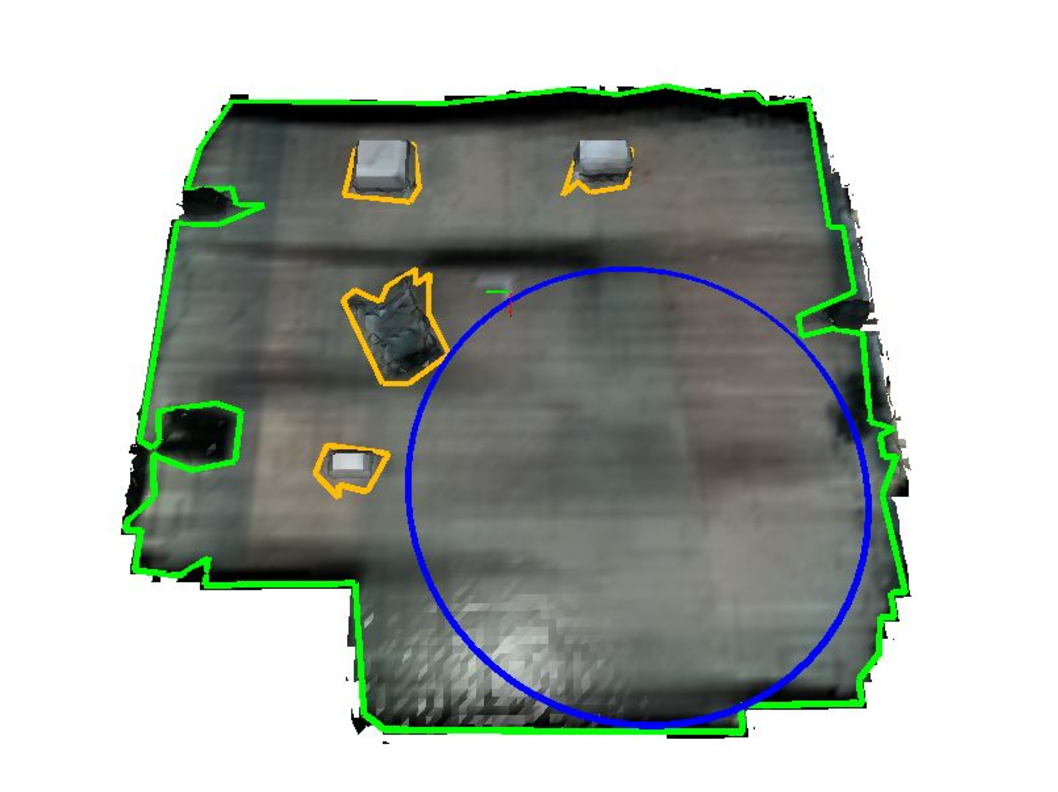
\includegraphics[page=1,clip,trim=2cm 0cm 2cm 0cm,width=.99\linewidth]{chapter_7_experiments/imgs/mesh_man_all.pdf}
    \caption{\label{fig:ch7_mesh_a}}
  \end{subfigure}
  \begin{subfigure}[t]{.30\linewidth}
    \centering  \includegraphics[page=2,clip,trim=2cm 0cm 2cm 0cm,width=.99\linewidth]{chapter_7_experiments/imgs/mesh_man_all.pdf}
    \caption{\label{fig:ch7_mesh_b}}
  \end{subfigure}
  
  \begin{subfigure}[t]{.33\linewidth}
    \centering  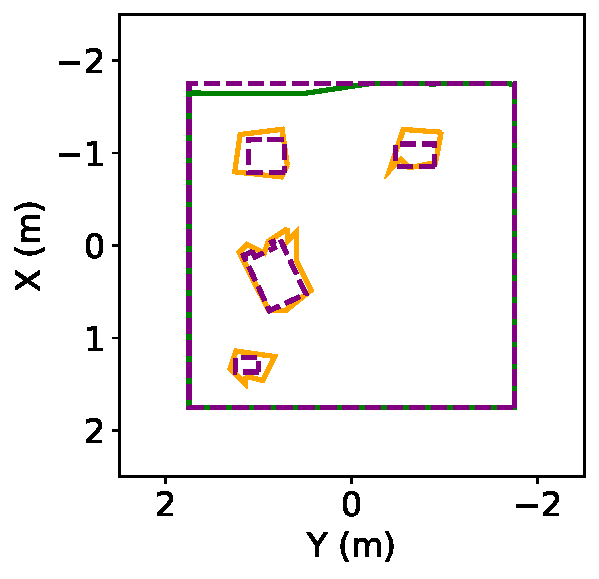
\includegraphics[clip,trim=0cm 0cm 0cm 0cm,width=.99\linewidth]{chapter_7_experiments/imgs/man_poly_1.pdf}
    \caption{\label{fig:ch7_man_poly_a}}
  \end{subfigure}
  \begin{subfigure}[t]{.33\linewidth}
    \centering  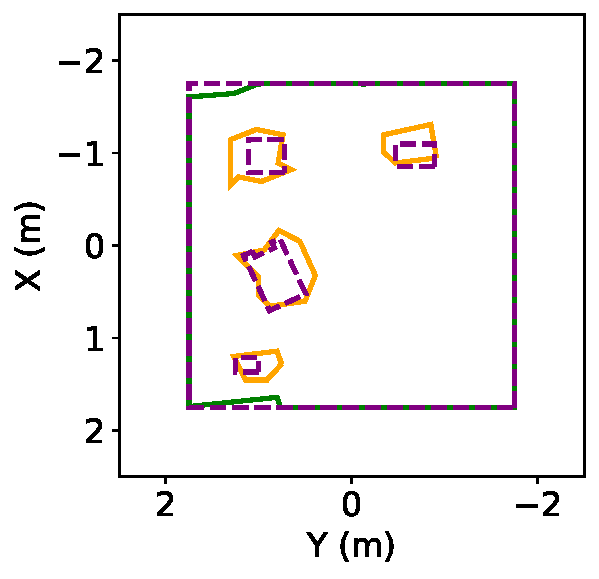
\includegraphics[clip,trim=0cm 0cm 0cm 0cm,width=.99\linewidth]{chapter_7_experiments/imgs/man_poly_3.pdf}
    \caption{\label{fig:ch7_man_poly_b}}
  \end{subfigure}
   \caption[Real-time constructed meshes and polygons during hand carry test]{(a,b) Examples of real-time constructed meshes, polygons, and touchdown points from two hand carry tests. Polygon shown in green/orange and touchdown circle in blue. (c,d) Comparisons of the ground truth polygon (dashed purple) versus extracted polygons.} \label{fig:ch7_mesh_handcarry}
%   (\subref{fig:ch7_mesh_a}, \subref{fig:ch7_mesh_b}) 
\end{figure}

Figures~\ref{fig:ch7_man_poly_a},\subref{fig:ch7_man_poly_b} display the same polygons shown in (a,b) but projected to the XY plane alongside the ground truth workspace previously shown in Figure\ref{fig:ch7_workspace_b}. The landable area and obstacles are accurately captured in both examples. Our methods intentionally slightly exaggerate the size of obstacles to provide a safety buffer for landing.  We provide quantitative accuracy results by calculating the \ac{IOU} of the extracted polygon and the ground truth workspace.  The mean \ac{IOU} for all five tests was $94.2\%$ which indicates that the surface extraction was highly accurate. There seems to be a small positional bias ($< .05m$) in obstacle placement which may be from inaccurate localization in the T265 tracking sensor. The is investigated more thoroughly in Section \ref{sec:ch7_results_t265_accuracy}.


\subsection{Flight Tests} \label{sec:ch7_results_flight}

Three flight tests were conducted with the sensor package payload. In all experiments a \ac{PIC} had manual control of the quadrotor to execute a flight path shown in Figure \ref{fig:ch7_flight_path}. This box pattern allowed full coverage of the workspace by the L515 LiDAR during the integration process. Emergency landing protocols were then activated which extracted a mesh of the environment, found the optimal touchdown point, and began autonomous trajectory generation, control and landing procedures. In all flight tests the drone successfully found the touchdown point and landed. Each flight took approximately 75 seconds.

\begin{figure}[!tb]
    \centering  
    \includegraphics[page=3,clip,trim=0cm 0cm 0cm 0cm,width=.45\linewidth]{chapter_7_experiments/imgs/ExperimentSetup.pdf}
    \caption[Flight path for scanning environment]{Flight path of drone when scanning the environment}\label{fig:ch7_flight_path}
\end{figure}

Figures~\ref{fig:ch7_flight_mesh_a}\subref{fig:ch7_flight_mesh_b} show the meshes generated in real-time from the flight experiments. We can see that the mesh, polygons, and touchdown are similarly accurate to the hand carry tests. Figures~\ref{fig:ch7_man_poly_a},\subref{fig:ch7_man_poly_b} show the extracted polygons projected to the XY plane and compared with the ground truth polygon of the workspace. The mean \ac{IOU} for all three flight tests was $92.3\%$, slightly lower than the $94.3$\% accuracy of the hand carry tests.  This may indicate that the T265 struggled with more precise localization in flight versus being hand carried. 


\begin{figure}[!htb]
  \centering
  \begin{subfigure}[t]{.30\linewidth}
    \centering  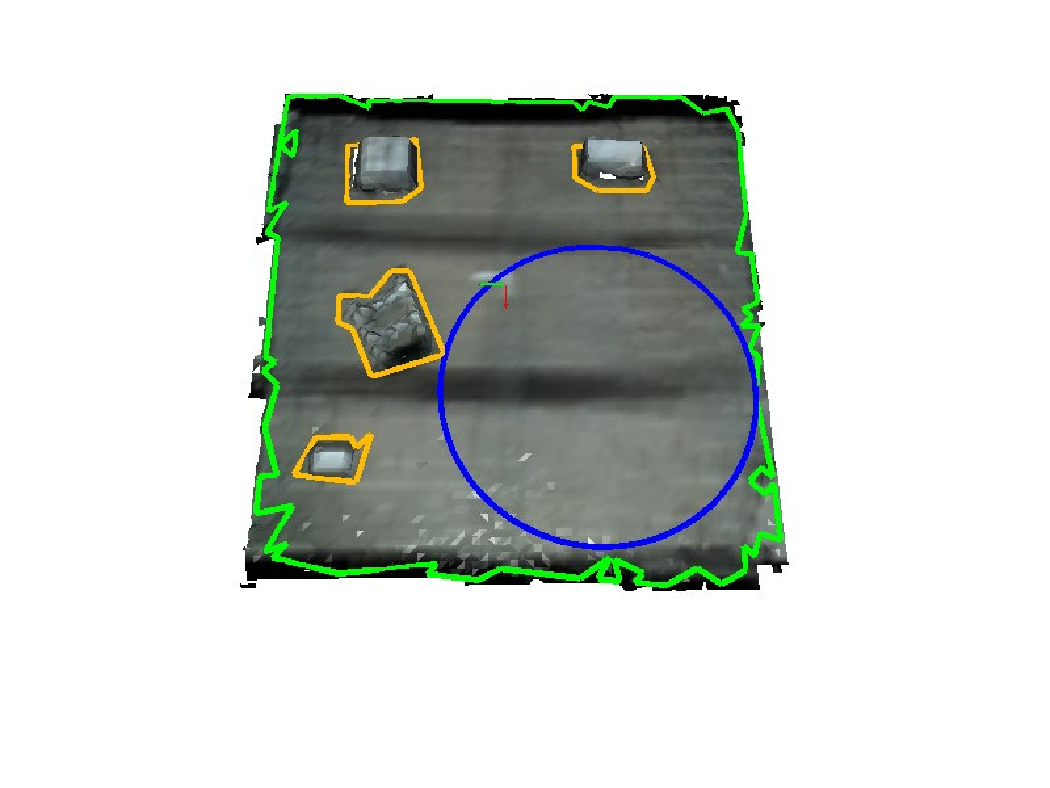
\includegraphics[page=1,clip,trim=4cm 3cm 4cm 1.4cm,width=.99\linewidth]{chapter_7_experiments/imgs/mesh_flight.pdf}
    \caption{\label{fig:ch7_flight_mesh_a}}
  \end{subfigure}
  \begin{subfigure}[t]{.30\linewidth}
    \centering  \includegraphics[page=2,clip,trim=4cm 3cm 4cm 1.4cm,width=.99\linewidth]{chapter_7_experiments/imgs/mesh_flight.pdf}
    \caption{\label{fig:ch7_flight_mesh_b}}
  \end{subfigure}
  
  \begin{subfigure}[t]{.35\linewidth}
    \centering  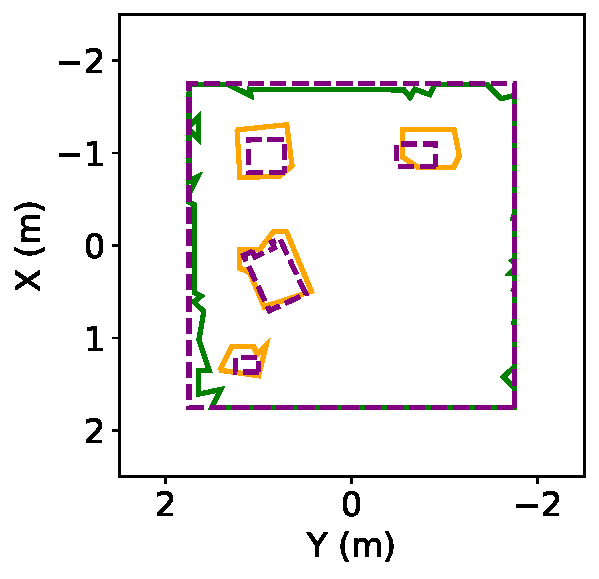
\includegraphics[clip,trim=0cm 0cm 0cm 0cm,width=.99\linewidth]{chapter_7_experiments/imgs/flight_poly_1.pdf}
    \caption{\label{fig:ch7_flight_poly_a}}
  \end{subfigure}
  \begin{subfigure}[t]{.35\linewidth}
    \centering  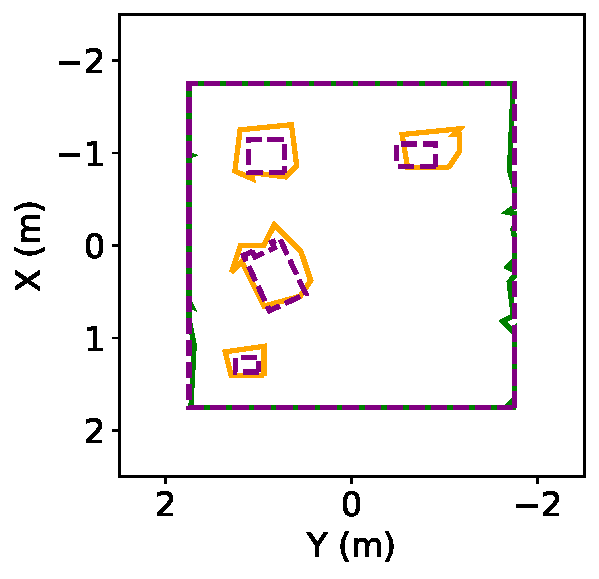
\includegraphics[clip,trim=0cm 0cm 0cm 0cm,width=.99\linewidth]{chapter_7_experiments/imgs/flight_poly_2.pdf}
    \caption{\label{fig:ch7_flight_poly_b}}
  \end{subfigure}
  \caption[Real-time constructed meshes and polygons during flight test]{(a,b) Examples of real-time constructed meshes, polygons, and touchdown points from two flight tests. Polygon shown in green/orange and touchdown circle in blue. (c,d) Comparisons of the ground truth polygon (purple) versus extracted polygons. }\label{fig:ch7_mesh_flight}
%   (\subref{fig:ch7_mesh_a}, \subref{fig:ch7_mesh_b}) 
\end{figure}




\subsection{Execution Time} \label{sec:ch7_results_execution_time}

The computation time for the major steps in our methods are calculated and presented in Table \ref{table:ch7_execution_time}. The table shows the mean execution time and standard deviation for all experiments conducted on both the low-power Odyseey x86 \ac{SBC} as well as a desktop computer. Both computers run the same software and data that was recorded for all experiments. The Odyssey board has an Intel J4105 processor with 4 Cores and 8 GB of RAM while the desktop is configured with a 12 core AMD 3900X processor with 32 GB of RAM. In both systems a maximum of 2 threads were used for parallelization in Polylidar3D for polygon extraction. All other steps are single threaded. 

For each test approximately 111 \ac{RGBD} frames were integrated into a voxel volume.  Once the volume is created, a triangular mesh of the environment is extracted.  Polylidar3D then extracts a polygon of the mesh, filters/simplifies it, and an optimal touchdown point is found. The Odyssey \ac{SBC} executed volume integration quick enough to match the 6 Hz stream of the LiDAR sensor. Additionally, our landing site selection software was able to find a safe landing site in less than 60 ms within the environment. In most cases the desktop computer is $\approx3$ times faster than the Odyssey \ac{SBC}. However, frame integration has a 10X performance degradation when using the Odyssey board in comparison to the desktop computer.  This can be seen not only from the average execution times but also the large standard deviation of 27ms. 

\begin{table}[H]
\centering
\caption{Mean and Standard Deviation of Execution Times (ms)}\label{table:ch7_execution_time}
\resizebox{\columnwidth}{!}{
\begin{tabular}{c@{\qquad}cc@{\qquad}ccc}
  \toprule 
  \multirow{2}{*}{\raisebox{-\heavyrulewidth}{\textbf{Computer}}} & \multicolumn{2}{c}{\textbf{Volume Integration}} & \multicolumn{3}{c}{\textbf{Landing Site Selection}} \\
  \cmidrule{2-6}
   &  \textbf{Integrate Frame} & \textbf{Extract Mesh} & \textbf{Extract Polygon} & \textbf{Filter Polygon} & \textbf{Touchdown Site} \\
  \midrule 
  Odyssey \ac{SBC} & $19.6 \pm 27.2 $ & $47.8 \pm 8.4$ & $18.3 \pm 2.9$ & $39.1 \pm 9.2$ & 0.2  \\
  Desktop     & $2.5 \pm 0.5$  & $16.9 \pm 2.6$ & $6.7 \pm 0.9$  & $14.0 \pm 5.1$ &  $0.1$  \\
  \bottomrule
\end{tabular}
}
\end{table}


\subsection{Position and Rotational Accuracy of T265}\label{sec:ch7_results_t265_accuracy}

% The Intel RealSense T265 utilizes an unknown closed source visual odometry algorithm with loop closure. A primary benefit is that the camera itself contains an on-board ASIC to perform all SLAM calculations to output the 6DOF pose. This reduces the computational burden for flight controllers or other companion boards. The product was released in 2020 with recent papers investigating its tracking performance \cite{ouerghi:hal-02567816, 10.1007/978-3-030-70740-8_14}. However, to the authors knowledge no accuracy results have been reported when mounted on \ac{sUAS} with motion capture for ground truth estimates.

This section provides accuracy results of the T265 pose predictions in comparison to the ground truth \ac{MCS}. The T265 predicted pose estimates are given an initial alignment to the ground truth trajectory following standard evaluation procedures in \cite{zhang_tutorial_2018}. Figure \ref{fig:ch7_flight_path_3d} shows the 3D trajectory of the drone in the first flight experiment using pose estimates from the \ac{MCS} (orange) and the T265 (blue). The predicted T265 trajectory closely follows \ac{MCS} but appears to drift away marginally after time. Figure \ref{fig:ch7_t265} provides individual graphs comparisons for the x, y, z, roll, pitch, and yaw estimates for this first flight experiment.

\begin{figure}[!ht]
    \centering  
    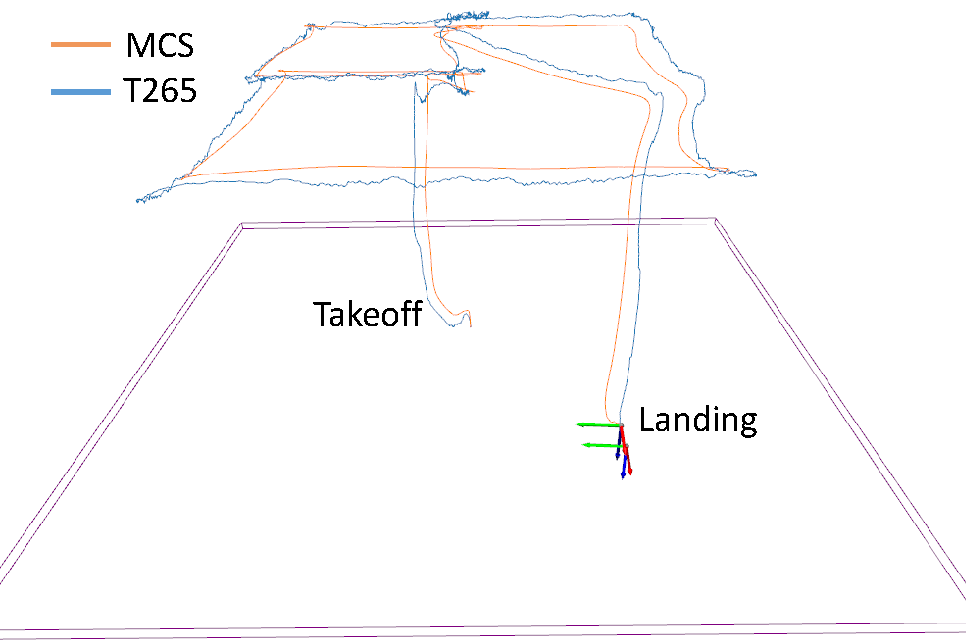
\includegraphics[page=1,clip,trim=0cm 0cm 0cm 0cm,width=.45\linewidth]{chapter_7_experiments/imgs/flight_path_t265_mcs.pdf}
    \caption[Trajectory of drone from Motion Capture System (MCS) versus T265]{Trajectory of Drone from Motion Capture System versus T265}\label{fig:ch7_flight_path_3d}
\end{figure}

\begin{figure}[!ht]
    \centering  
    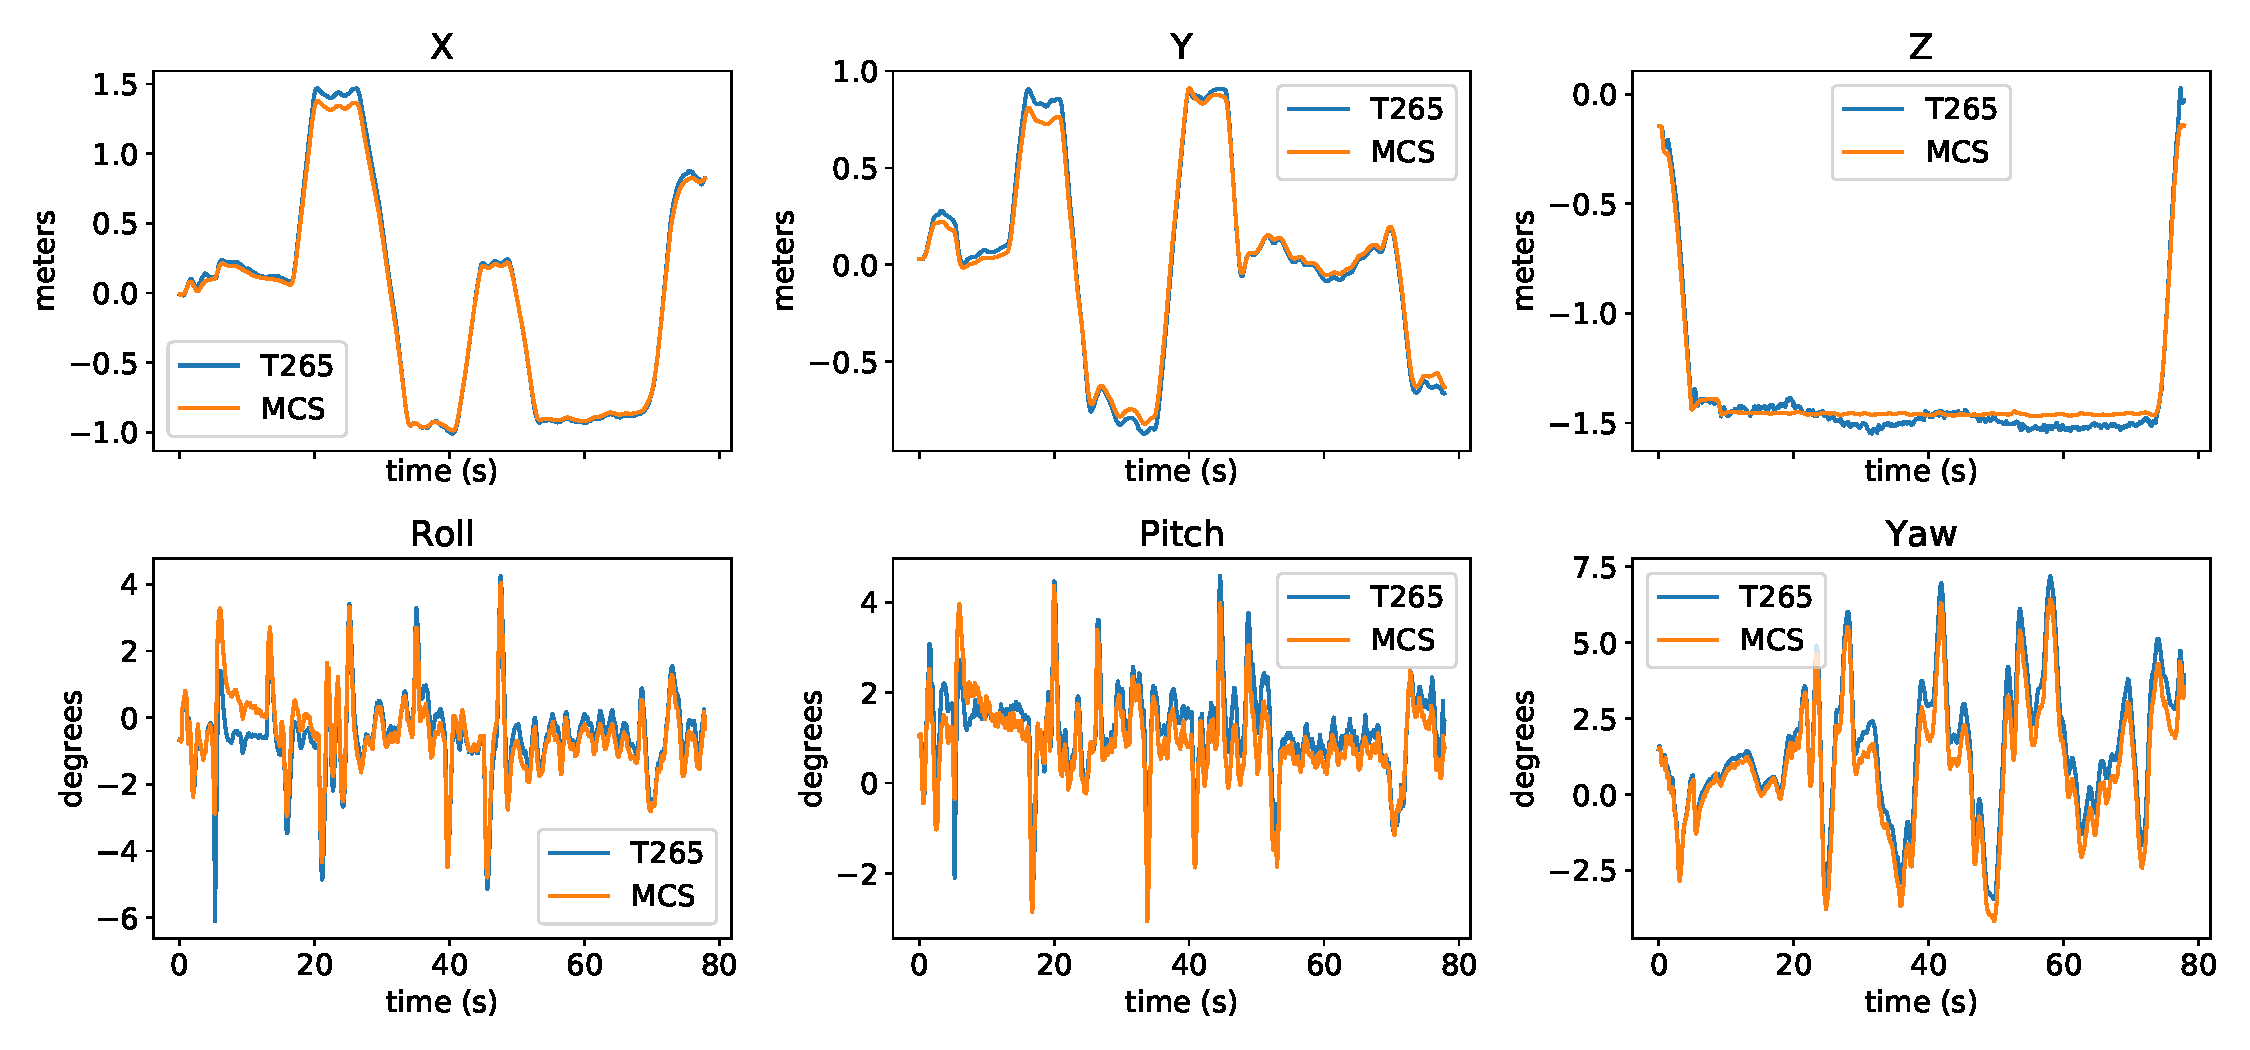
\includegraphics[page=1,clip,trim=0cm 0cm 0cm 0cm,width=.95\linewidth]{chapter_7_experiments/imgs/t265_gt_graphs_v2.pdf}
    \caption[Comparison of Motion Capture System (MCS) versus T265]{Flight \#1 comparison of Motion Capture System (MCS) versus T265}\label{fig:ch7_t265}
\end{figure}
The mean absolute trajectory error is calculated for each flight and displayed in Table \ref{table:ch7_ate}. The position and rotation error are computed following procedures in \cite{zhang_tutorial_2018}. The average length of each flight experiment is approximately 17.2m. The position and rotational error is low for the the first and second flight but markedly higher in the third flight. The third flight lost altitude tracking near the beginning of the fight but recovered after 5 seconds.

\begin{table}[h]
\centering
\caption{Mean Absolute Trajectory Error (ATE) for T265}\label{table:ch7_ate}
\begin{tabular}{@{}lccc@{}}
\toprule
Trial    & Length (m) & Position Mean ATE (m) & Rotation Mean ATE (deg) \\ \midrule
Flight \#1 & 17.1       & 0.11                  & 0.98                    \\
Flight \#2 & 16.6       & 0.10                  & 1.03                    \\
Flight \#3 & 17.9       & 0.35                  & 3.7                     \\ \bottomrule
\end{tabular}
\end{table}


\section{Conclusion and Future Work}

Multiple experiments were conducted to validate our proposed methods for real-time landing site identification and selection. We developed a sensor-package that holds an Intel RealSense L515 LiDAR, RealSense T265 Tracking Camera, and an Odyseey x86 \acf{SBC}. Together they provide depth data, localization and mapping, and the computational power necessary for our landing software. The sensor package was both hand-carried and flown with a quadrotor in an obstacle cluttered indoor environment. Accurate meshes of the environment were generated in real-time for which landing sites were extracted as polygons. The polygons representing safe landable area were compared against the ground truth map and found to be highly accurate. In every experiment a safe landing zone was found which correctly minimized risk. 

Future experimental work should be conducted at integrating a semantic neural network with Polylidar3D as proposed in Chapter \ref{ch:landingsim}. Data of real-world and synthetic environments should be captured and labelled to train the proposed network. The Odyssey board should be swapped out with a \ac{SBC} with an on-board \ac{GPU} to provide minimal inference time for semantic segmentation.









